\documentclass{llncs}

\usepackage{url}
\usepackage{bar}
\usepackage{comment}
\usepackage{graphicx}

%include polycode.fmt
%include supero.fmt

\newenvironment{fig}
    {\begin{figure}[tbp]\hrule}
    {\end{figure}}

\newcommand{\figend}{\hrule}
\newcommand{\perc}{\%
    }
\newcommand{\noexample}{\hfill$\Box$}

\newcommand{\generalise}{\bowtie}


\begin{document}

% COMMENTS FROM COLIN
% to fix before post-proceedings
%
% More story - abstract - on 8 benchmarks
% Intro - contributions
% Figure on how to apply O, Fig 3 caption improvements
% Reason for GHC increasing in wc benchmarks
% More benchmarks - and larger
% Related work - Dunstall 1981, Turin, Supercompilation
% Ignore low-level optimisation
% Specialisation, whole program
% Termination - fix

\title{A Supercompiler for Core Haskell}

\author{Neil Mitchell and Colin Runciman}

\institute{University of York, UK, \url{http://www.cs.york.ac.uk/~ndm}}

\maketitle              % typeset the title of the contribution

\begin{abstract}
Haskell is a functional language, with features such as higher order functions and lazy evaluation, which allow succinct programs. These high-level features present many challenges for optimising compilers. We report practical experiments using novel variants of \textit{supercompilation}, with special attention to let bindings and the generalisation technique.
\end{abstract}

\section{Introduction}

Haskell \cite{haskell} can be used in a highly declarative manner, to express specifications which are themselves executable. Take for example the task of counting the number of words in a file read from the standard input. In Haskell, one could write:

\begin{code}
main = print . length . words =<< getContents
\end{code}

From right to left, the |getContents| function reads the input as a list of characters, |words| splits this list into a list of words, |length| counts the number of words, and finally |print| writes the value to the screen.

An equivalent C program is given in Figure \ref{fig:c_words}. Compared to the C program, the Haskell version is more concise and more easily seen to be correct. Unfortunately, the Haskell program (compiled with GHC \cite{ghc}) is also three times slower than the C version (compiled with GCC). This slowdown is caused by several factors:

\begin{fig}
\bigskip
\begin{verbatim}
int main()
{
	int i = 0;
	int c, last_space = 1, this_space;
	while ((c = getchar()) != EOF) {
		this_space = isspace(c);
		if (last_space && !this_space)
			i++;
		last_space = this_space;
	}
	printf("%i\n", i);
	return 0;
}
\end{verbatim}
\figend
\caption{Word counting in C.}
\label{fig:c_words}
\end{fig}

\begin{description}
\item[Intermediate Lists] The Haskell program produces and consumes many intermediate lists as it computes the result. The |getContents| function produces a list of characters, |words| consumes this list and produces a list of lists of characters, |length| then consumes the outermost list. The C version uses no intermediate data structures.
\item[Functional Arguments] The |words| function is defined using the |dropWhile| function, which takes a predicate and discards elements from the input list until the predicate becomes true. The predicate is passed as an invariant function argument in all applications of |dropWhile|.
\item[Laziness and Thunks] The Haskell program proceeds in a lazy manner, first demanding one character from |getContents|, then processing it with each of the functions in the pipeline. At each stage, a lazy thunk for the remainder of each function is created.
\end{description}

Using the optimiser developed in this paper, named Supero, we can eliminate all these overheads. We obtain a program that performs \textit{faster} than the C version. The optimiser is based around the techniques of supercompilation \cite{supercompilation}, where some of the program is evaluated at compile time, leaving an optimised residual program.

Our goal is an automatic optimisation that makes high-level Haskell programs run as fast as low-level equivalents, eliminating the current need for hand-tuning and low-level techniques to obtain competitive performance. We require no annotations on any part of the program, including the library functions.

\subsection{Contributions}

\begin{itemize}
\item To our knowledge, this is the first time supercompilation has been applied to Haskell. \item We make careful study of the let expression, something absent from the Core language of many other papers on supercompilation.
\item We present an alternative generalisation step, based on a homeomorphic embedding \cite{leuschel:homeomorphic}.
\end{itemize}

\subsection{Roadmap}

We first introduce a Core language in \S\ref{sec:core}, on which all transformations are applied. Next we describe our supercompilation method in \S\ref{sec:optimisation}. We then give a number of benchmarks, comparing both against C (compiled with GCC) in \S\ref{sec:c_results} and Haskell (compiled with GHC) in \S\ref{sec:haskell_results}. Finally, we review related work in \S\ref{sec:related} and conclude in \S\ref{sec:conclusion}.

\section{Core Language}
\label{sec:core}

\begin{fig}
\begin{code}
expr  =  v                                          {-" \text{  variable} "-}
      |  c                                          {-" \text{  constructor} "-}
      |  f                                          {-" \text{  function} "-}
      |  x ys_                                      {-" \text{  application} "-}
      |  \vs_ -> x                                  {-" \text{  lambda abstraction} "-}
      |  let v = x in y                             {-" \text{  let binding} "-}
      |  case x of {p_1 -> y_1 ; ... ; p_n -> y_n}  {-" \text{  case expression} "-}

pat   =  c vs_
\end{code}

Where |v| ranges over variables, |c| ranges over constructors, |f| ranges over functions, |x| and |y| range over expressions and |p| ranges over patterns.
\bigskip
\figend
\caption{Core syntax}
\label{fig:core}
\end{fig}

Our supercompiler uses the Yhc-Core language \cite{me:yhc_core}. The expression type is given in Figure \ref{fig:core}. A program is a mapping of function names to expressions. Our Core language is higher order and lazy, but lacks much of the syntactic sugar found in Haskell. Pattern matching occurs only in case expressions, and all case expressions are exhaustive. All names are fully qualified. Haskell's type classes have been removed using the dictionary transformation \cite{wadler:type_classes}.

The Yhc compiler, a fork of nhc \cite{nhc}, can output Core files. Yhc can also link in all definitions from all required libraries, producing a single Core file representing a whole program.

The primary difference between Yhc-Core and GHC-Core \cite{ghc_core} is that Yhc-Core is untyped. The Core is generated from well-typed Haskell, and is guaranteed not to fail with a type error. All the transformations could be implemented equally well in a typed Core language, but we prefer to work in an untyped language for simplicity of implementation.

In order to avoid accidental variable name clashes while performing transformations, we demand that all variables within a program are unique. All transformations may assume this invariant, and must maintain it.

\begin{fig}
\vspace{2mm}
\begin{tabular}{rcl}
|split(v)| & |=| & |(v, [])| \\
|split(c)| & |=| & |(c, [])| \\
|split(f)| & |=| & |(f, [])| \\
|split(x ys_)| & |=| & |(bullet {-"\text{ } \overline{\bullet} "-}, x:ys_)| \\
|split(\vs_ -> x)| & |=| & |(\vs_ -> bullet, x)| \\
|split(let v = x in y)| & |=| & |(let v = bullet in bullet, [x,y])| \\
|split(case x of {p_1 \! -> \! y_1 ; ... ; p_n \! -> \! y_n})| & |=| & |(case {-"\hspace{-1mm}"-} bullet {-"\hspace{-1mm}"-} of {p_1 \! -> \! bullet ; ... ; p_n \! -> \! bullet}, [x, y_1, ... ,y_n])|
\end{tabular}
\vspace{2mm}
\figend
\caption{The |split| function, returning a spine and all subexpressions.}
\label{fig:split}
\end{fig}

We define the |split| function in Figure \ref{fig:split}, which splits an expression into a pair of its spine and its immediate subexpressions. The $\bullet$ markers in the spine indicate the positions from which subexpressions have been removed. We define the |join| operation to be the inverse of |split|, taking a spine and a list of expressions, and producing an expression.

\section{Supercompilation}
\label{sec:optimisation}

Our supercompiler takes a Core program as input, and produces an equivalent Core program as output. To improve the program we do not make small local changes to the original, but instead \textit{evaluate it} so far as possible at compile time, leaving a \textit{residual program} to be run.

\begin{fig}
\begin{code}
supercompile()
    seen := {}
    bind := {}
    tie({}, main)
\end{code}

\vspace{-6mm}

\begin{tabular}{p{6.9cm}p{5cm}}
\begin{code}
tie(rho, x)
    if x `notElem` seen then
        seen := seen `union` {x}
        bind := bind `union` {psi\!!(x) = \ fv\!!(x) -> drive\!!(rho,x)}
    {-" \textsf{\textbf{endif}} "-}
    {-" \textsf{\textbf{return }} "-} (psi\!!(x) fv\!!(x))
\end{code}
&
\begin{code}
drive(rho, x)
    if terminate\!!(rho, x) then
        (a,b) = split\!!(generalise\!!(x))
        {-" \textsf{\textbf{return }} "-} join\!!(a, map (tie rho) b)
    else
        {-" \textsf{\textbf{return }} "-} drive\!!(rho `union` {x}, unfold(x))
\end{code}
\end{tabular}

\vspace{-3mm}

Where |psi| is a mapping from expressions to function names, and |fv\!!(x)| returns the free variables in |x|. This code is parameterised by: |terminate| which decides whether to stop supercompilation of this expression; |generalise| which generalises an expression before residuation; |unfold| which chooses a function application and unfolds it.
\vspace{3mm}
\figend
\caption{The |supercompile| function.}
\label{fig:supercompile}
\end{fig}

The general method of supercompilation is shown in Figure \ref{fig:supercompile}. Each function in the output program is an optimised version of some associated expression in the input program. Supercompilation starts at the |main| function, and supercompiles the expression associated with |main|. Once the expression has been supercompiled, the outermost element in the expression becomes part of the residual program. All the subexpressions are assigned names, and will be given definitions in the residual program. If any expression (up to alpha renaming) already has a name in the residual program, then the same name is used. Each of these named inner expressions are then supercompiled as before.

\begin{comment}
\begin{fig}
\begin{code}
_O\<case x of alts_  \> =  case _O\<x\> \? of alts_
_O\<let v = x in y   \> =  let v = _O\<x\> \? in _O\<y\>
_O\<x y              \> =  _O\<x\> \? y
_O\<f                \> =  unfold f  , where f {-" \hbox{ is a non-primitive, non-CAF function} "-}
                        =  f         , otherwise
_O\<v                \> =  v
_O\<c                \> =  c
_O\< \v -> x         \> =  \v -> x
\end{code}
\figend
\caption{Optimisation rules.}
\label{fig:optimise}
\end{fig}
\end{comment}

\begin{fig}
\begin{code}
case (case x of {p_1 -> y_1 ; ... ; p_n -> y_n}) of alts_
    => case x of  {  p_1  -> case y_1 of alts_
                  ;  ...
                  ;  p_n  -> case y_n of alts_ }

case c xs_ of {... ; c vs_ -> y ; ...}
    => y[vs_/xs_]

case v of {... ; c vs_ -> x ; ...}
    => case v of {... ; c vs_ -> x[v/c vs_]; ...}

case (let v = x in y) of alts_
    => let v = x in case y of alts_

(let v = x in y) z
    => let v = x in y z

(case x of {p_1 -> y_1 ; ... ; p_n -> y_n}) z
    => case x of {p_1 -> y_1 z ; ... ; p_n -> y_n z}

(\v -> x) y
    => let v = y in x

let v = x in (case y of {p_1 -> y_1 ; ... ; p_n -> y_n})
    => case y of  {  p_1  -> let v = x in y_1
                  ;  ...
                  ;  p_n  -> let v = x in y_n}
    where v {-" \hbox{is not used in } "-} y

let v = x in y
    => y[v/x]
    where x {-" \hbox{is a lambda, a variable, or } "-} v {-" \hbox{is used once in } "-} y

let v = c x_1 ... x_n in y
    =>  let v_1 = x_1 in
        ...
        let v_n = x_n in
        y[v/c v_1 ... v_n]
    where v_1 ... v_n {-" \hbox{ are fresh} "-}
\end{code}
\figend
\caption{Simplification rules.}
\label{fig:simplify}
\end{fig}

The supercompilation of an expression proceeds by repeatedly inlining a function application until some termination criterion is met. Once the termination criterion holds, the expression is generalised before the outer spine becomes part of the residual program and all immediate subexpressions are assigned names. After each inlining step, the expression is simplified using the rules in Figure \ref{fig:simplify}. There are three key decisions in the supercompilation of an expression:

\begin{enumerate}
\item Which function to inline.
\item What termination criterion to use.
\item What generalisation to use.
\end{enumerate}

The original Supero work \cite{me:supero_ifl} inlined following evaluation order (with the exception of let expressions), used a bound on the size of the expression to ensure termination, and performed no generalisation. First we give examples of our supercompiler in use, then we return to examine each of the three choices we have made.

\subsection{Examples of Supercompilation}

\subsubsection{Example 1: Supercompiling and Specialisation}\hfill

\begin{code}
main as = map (\b -> b + 1) as

map f cs = case  cs of
                 []    -> []
                 d:ds  -> f d : map f ds
\end{code}

There are two primary inefficiencies in this example: (1) the |map| function passes the |f| argument invariantly in every call; (2) the application of |f| is more expensive than if the function was known in advance.

The supercompilation proceeds by first assigning a new unique name (we choose |h0|) to |map (\b -> b + 1) as|, providing parameters for each of the free variables in the expression, namely |as|. We then choose to expand |map|, and invoke the simplification rules:

\begin{code}
h0 as  = map (\b -> b + 1) as

       = case  as of
               []    -> []
               d:ds  -> d+1 : map (\b -> b + 1) ds
\end{code}

We now have a |case| with a variable as the scrutinee at the root of the expression, which cannot be reduced further, so we residuate the spine. When processing the expression |map (\b -> b + 1) ds| we spot this to be an alpha renaming of the body of an existing generated function, namely |h0|, and use this function:

\begin{code}
h0 as = case  as of
              []    -> []
              d:ds  -> d+1 : h0 ds
\end{code}

We have now specialised the higher-order argument, passing less data at runtime.\noexample

\subsubsection{Example 2: Supercompiling and Deforestation}\hfill

The deforestation transformation \cite{wadler:deforestation} removes intermediate lists from a traversal. A similar result is obtained by applying supercompilation, as shown here. Consider the operation of mapping |(*2)| over a list and then mapping |(+1)| over the result. The first |map| deconstructs one list, and constructs another. The second does the same.

\begin{code}
main as = map (\b -> b+1) (map (\c -> c*2) as)
\end{code}

We first assign a new name for the body of |main|, then choose to expand the outer call to |map|:

\begin{code}
h0 as = case  map (\c -> c*2) as of
              []    -> []
              d:ds  -> y+1 : map (\b -> b+1) ds
\end{code}

Next we choose to inline the |map| scrutinised by the case, then perform the |case|/|case| simplification, and finally residuate:

\begin{code}
h0 as  = case  (case  as of
                      []    -> []
                      e:es  -> e*2 : map (\c -> c*2) es) of
               []    -> []
               d:ds  -> y+1 : map (\b -> b+1) ds

       = case  as of
               []    -> []
               d:ds  -> (y*2)+1 : map (\b -> b+1) (map (\c -> c*2) ds)

       = case  as of
               []    -> []
               d:ds  -> (y*2)+1 : h0 ds
\end{code}

Both intermediate lists have been removed, and the functional arguments to |map| have both been specialised.  \noexample

\subsection{Which function to inline}

During the supercompilation of an expression, at each step some function needs to be inlined. Which to choose? In most supercompilation work the choice is made following the runtime semantics of the program. But in a language with let expressions this may be inappropriate. If a function in a let binding is inlined, its application when reduced may be simple enough to substitute in the let body. However, if a function in a let body is inlined, the let body may now only refer to the let binding once, allowing the binding to be substituted. Let us take two expressions, based on intermediate steps obtained from real programs (word counting and prime number calculation respectively):

\begin{tabular}{p{5cm}p{5cm}}
\begin{code}
let x = (==) $ 1
in x 1 : map x ys
\end{code}
&
\begin{code}
let x = repeat 1
in const 0 x : map f x
\end{code}
\end{tabular}

In the first example, inlining |($)| in the let binding gives |(\x -> 1 == x)|, which is now simple enough to substitute for |x|, resulting in |(1 == 1 : map (\x -> 1 == x) ys)| after simplification. Now |map| can be specialised appropriately. Alternatively, expanding the |map| repeatedly would keep increasing the size of expression until the termination criterion was met, aborting the supercompilation of this expression without achieving specialisation.

Taking the second example, |repeat| can be inlined indefinitely. However, by unfolding the |const| we produce |let x = repeat 1 in 0 : map f x|. Since |x| is only used once we substitute it to produce |(0 : map f (repeat 1))|, which can be deforested.

Unfortunately these two examples seem to suggest different strategies for unfolding -- unfold in the let binding or unfold in the let body. However, they do have a common theme -- unfold the function that cannot be unfolded infinitely often. Our strategy can be defined by the |unfold| function:

\begin{code}
unfold x = head (filter (not . terminate) xs ++ xs ++ [x])
    where xs = unfolds x

unfolds f | f {-" \text{ is a function} "-} = [inline f]
unfolds x =  [join spine (sub |+ (i, y))
             |let (spine, sub) = split x
             ,i <- [0..length sub], y <- unfolds (sub !! i) ]
    where xs |+ (i,x) = zipWith (\j y -> if i == j then x else y) [0..] xs
\end{code}

The |unfolds| function computes all possible one-step inlinings, using an in-order traversal of the abstract syntax tree. The |unfold| function chooses the first unfolding which does not cause the supercompilation to terminate. If no such expression exists, the first unfolding is chosen.

\subsection{The Termination Criterion}

The original Supero program used a size bound on the expression to determine when to stop. The problem with a size bound is that different programs require different bounds to ensure both timely completion at compile-time and efficient residual programs. Indeed, within a single program, there may be different elements requiring different size bounds -- a problem exacerbated as the size and complexity of a program increases.

We use the termination criterion suggested by S{\o}rensen and Gl{\"u}ck \cite{sorensen:supercompilation} -- homeomorphic embedding. An expression $x$ is an embedding of $y$, written $x \unlhd y$, if the relationship can be inferred by the rules:

\noindent\begin{tabular}{p{5cm}p{5cm}}
\[\frac{\text{dive}(x,y)}{x \unlhd y}\] \vspace{-8mm}
&
\[\frac{\text{couple}(x,y)}{x \unlhd y}\] \vspace{-8mm}
\\
\[\frac{s \unlhd t_i \text{ for some } |i|}{\text{dive}(s, \sigma(t_1,\ldots,t_n))} \]
&
\[\frac{\sigma_1 \sim \sigma_2,
        s_1 \unlhd t_1, \ldots , s_n \unlhd t_n}
       {\text{couple}(\sigma_1 (s_1,\ldots,s_n), \sigma_2 (t_1,\ldots,t_n))}
\]
\end{tabular}

The homeomorphic embedding uses the relations dive and couple. The dive relation checks if the left term is contained as a child of the right term, while the couple relation checks if both terms have the same outer shell. We use $\sigma$ to denote the spine of an expression, with $s_1,\ldots,s_n$ being its subexpressions. We test for equivalence of $\sigma_1$ and $\sigma_2$ using the $\sim$ relation, a weakened form of equality where all variables are considered equal. We terminate the supercompilation of an expression |y| if on the chain of reductions from |main| to |y| we have encountered an expression |x| such that $x \unlhd y$.

In addition to using the homeomorphic embedding, we also terminate if further unfolding cannot yield any improvement to the root of the expression. For example, if the root of an expression is a constructor application, no further unfolding will change the root constructor. When terminating for this reason, we always residuate the outer spine of the expression, without applying any generalisation.

\subsection{Generalisation}

When the termination criterion has been met, it is necessary to discard information about the current expression, so that the supercompilation terminates. We always residuate the outer spine of the expression, but first we attempt to generalise the expression so that the information lost is minimal. The paper by S{\o}rensen and Gl{\"u}ck provides a method for generalisation, which works by taking the most specific generalisation of the current expression and expression which is a homeomorphic embedding of it.

The most specific generalisation of two expressions $s$ and $t$, $\text{msg}(s,t)$, is produced by applying the following rewrite rule to the initial triple $(x,\{x=s\},\{x=t\})$, resulting in a common expression and two sets of bindings.

\[
\left( \begin{array}{lcl}
	t_g \\
	\{x = \sigma(s_1,\ldots,s_n)\} & \cup & \theta_1 \\
	\{x = \sigma(t_1,\ldots,t_n)\} & \cup & \theta_2
	\end{array} \right)
\rightarrow
\left( \begin{array}{lcl}
	t_g[x / \sigma(y_1,\ldots,y_n)] \\
	\{y_1 = s_1,\ldots,y_n = s_n\} & \cup & \theta_1 \\
	\{y_1 = t_1,\ldots,y_n = t_n\} & \cup & \theta_2
	\end{array} \right)
\]

Our generalisation is characterised by $x \bowtie y$, which produces an expression equivalent to $y$, but similar in structure to $x$.

\vspace{-3mm}
\noindent\begin{tabular}{p{7cm}p{5cm}}
\begin{code}
{-" x \bowtie \sigma^*(y), \text{if dive}(x,\sigma^*(y)) \wedge \text{couple}(x,y) "-}
        let f = \vs_ -> x in {-" \sigma^* "-}(f vs)
        {-" \text{where } "-}vs_{-" = \text{fv}(y) \backslash \text{fv}(\sigma^*(y)) "-}
\end{code}
&
\begin{code}
{-" x \bowtie y, \text{if couple}(x,y) "-}
        let {-" \theta_2 "-} in {-" t_g "-}
        {-" \text{where }(t_g,\theta_1,\theta_2) = \text{msg}(x,y) "-}
\end{code}
\end{tabular}
\vspace{-3mm}

The fv function in the first rule calculates the free variables of an expression, and $\sigma^*(y)$ denotes a subexpression $y$ within a containing context $\sigma^*$. The first rule applies if the homeomorphic embedding first applied the dive rule. The idea is to descend to the element which matched, and then promote this to the top-level using a lambda. The second rule applies the most specific generalisation operation if the coupling rule was applied first. We now show an example where most specific generalisation fails to produce the ideal generalised version.

\subsubsection{Example 3}\hfill

\begin{code}
case  putStr (repeat '1') r of
      (r, _) -> (r, ())
\end{code}

This expression (which we name $x$) prints an infinite stream of 1's. The pairs and |r|'s correspond to the implementation of GHC's IO Monad \cite{spj:awkward_squad}. After several unrollings, we obtain the expression (named $x'$):

\begin{code}
case  putChar '1' r of
      (r, _) -> case  putStr (repeat '1') r of
                      (r, _) -> (r, ())
\end{code}

The homeomorphic embedding $x \unlhd x'$ matches, detecting an occurrence of the |case putStr \? ...| expression, and the supercompilation of $x'$ is stopped. The most specific generalisation rule is applied as $\text{msg}(x,x')$ and produces:

\begin{code}
let  a = putChar
     b = '1'
     c = \r -> case  putStr (repeat '1') r of
                     (r, _) -> (r, ())
in case  a b r of
         (r, _) -> c r
\end{code}

The problem is that msg works from the top, looking for a common root of both expression trees. However, if the first rule applied by $\unlhd$ was dive, the roots may be unrelated. Using our generalisation, $x \bowtie x'$:

\begin{code}
let x = \r -> case  putStr (repeat '1') r of
                    (r, _) -> (r, ())
in case  putChar '1' r of
         (r, _) -> x r
\end{code}

Our generalisation is superior because it has split out the |putStr| application \textit{without} lifting the |putChar| application or the constant |'1'|. The |putChar| application can now be supercompiled further in the context of the case expression.\noexample



\begin{comment}
Optimisation uses the |_O| rules in Figure \ref{fig:optimise}, and the simplification rules in Figure \ref{fig:simplify}. We define |_OO| to be the result of applying both |_O| and the simplification rules until no further changes are made. Optimisation is like evaluation, but stops if the expression to reduce is a free variable, a constructor, a primitive, or a CAF (constant applicative form -- see \S\ref{sec:caf} for more details). The one difference is that in a |let| expression the bound expression and the inner expression are \textit{both} optimised -- see \S\ref{sec:let} for the reasons. The simplification rules are all standard, and similar rules would be found in most optimising compilers.

\subsubsection{Example 1} \hfill

\begin{code}
main = \xs -> map inc xs

map = \f -> \xs -> case  xs of
                         []    -> []
                         y:ys  -> f y : map f ys

inc = \x -> x+1
\end{code}

This program defines a |main| function which increments each value in the list by one. Our |main| function is not a valid Haskell program, as it has the wrong type, but serves to illustrate the techniques. Note that |f| is passed around at runtime, when it could be frozen in at compile time. By following the optimisation procedure we end up with:

\begin{code}
main = \xs -> case  xs of
                    []    -> []
                    y:ys  -> f0 y ys

f0 = \y -> \ys -> (y+1) : main ys
\end{code}

And finally by performing some trivial inlining we can obtain:

\begin{code}
main = \xs -> case  xs of
                    []    -> []
                    y:ys  -> (y+1) : main ys
\end{code}

The residual program is now optimised -- there is no runtime passing of the |inc| function, only a direct arithmetic operation. \noexample

\subsubsection{Example 2} \hfill \vspace{2mm}

\noindent Our next example shows how our optimisation rules can carry out list deforestation \cite{wadler:deforestation}.

\begin{code}
main xs = map (+1) (map (*2) xs)

map f xs = case  xs of
                 []    -> []
                 y:ys  -> f y : map f ys
\end{code}

The main definition is transformed (after trivial inlining) into:

\begin{code}
main xs = case  xs of
                []    -> []
                y:ys  -> (y*2)+1 : main ys
\end{code}

\noindent The intermediate list has been removed, and the higher order functions eliminated by specialisation.\noexample


\subsection{Termination}
\label{sec:termination}

A problem with the method as presented so far is that it may not terminate. There are several ways that non-termination can arise. We consider, and eliminate, each in turn.

\subsubsection{Infinite Unfolding}

Consider the definition:

\begin{code}
name = \x -> name x
\end{code}

If the expression |name x| was being optimised then the optimisation function |_OO| would not terminate. We can solve this problem by either bounding the number of unfoldings, or by keeping a list of previously encountered intermediate expressions in |_OO|. In practice, this situation is rare, and either choice is acceptable. We choose to bound the number of unfoldings. A large limiting value is used, which does not impact either compilation time or memory consumption in the common case.

\subsubsection{Accumulating parameters}

Consider the definition:

\begin{code}
reverseAcc = \xs -> \ys -> case  xs of
                                 []    -> []
                                 z:zs  -> reverseAcc zs (z:ys)
\end{code}

This function is the standard |reverse| function, with an accumulator. The problem is that successive iterations of the optimisation produce progressively larger subexpressions. A definition is first created for |reverseAcc _ _|, then for |reverseAcc _ (_:_)|, then |reverseAcc _ (_:_:_)|. The residual program is infinite.

The solution is to bound the size of the input expression associated with each definition in the residual program. The size of the expression being optimised can be reduced by lifting subexpressions into a let binding, then placing this let binding in the residual program. By bounding the size of the expression, we bound the number of functions in the residual program.

If the bound is too high, optimisation takes too long and the residual program is excessively large. If the bound is too low then too little is achieved by optimisation. We return to the issue of the size of this bound in \S\ref{sec:results_bound}.

\subsubsection{Direct Repetition}
\label{sec:direct}

We claim that |_OO| terminates with bounded unfoldings and bounded expression size. It is often useful to detect an expression which appears to be repeating, and preemptively bound it. Consider the |reverseAcc| example -- the recursive pattern is an instance of \textit{direct repetition}. Let |alpha| be a context, and |alpha <^ e ^>| be the result of substituting |e| for the hole in the context |alpha|. An expression |x| is directly repeating if |x ~= alpha <^ alpha <^ beta ^> ^>| where |beta| is an expression, |alpha| is a non-empty context and |~=| is equality where all variables are considered equal.

\subsubsection{Example 3} \hfill\vspace{2mm}

\noindent The following expressions have direct repetition.

\begin{code}
x:y:xs   where alpha = x:hole  , beta = xs
f (f x)  where alpha = f hole  , beta = x
case x_1 of {[] -> nil ; y:ys -> case x_2 of {[] -> nil ; z:zs -> cons}}
    where alpha = case x_1 of {[] -> nil; y:ys -> hole}, beta = cons
\end{code}
\noexample

If direct repetition is encountered, then the repeating expression is lifted to a top-level let binding, and output directly into the residual program.

\subsubsection{Example 4} \hfill\vspace{2mm}

\noindent Take the |reverseAcc| example. During optimisation, the expression becomes:

\begin{code}
reverseAcc xs (y_1:y_2:ys)
\end{code}

\noindent The second argument to |reverseAcc| is an instance of direct repetition, and is lifted to a let binding.

\begin{code}
let v = y_1:y_2:ys
in reverseAcc xs v
\end{code}

\noindent Now the expression bound at the let, and the inner expression, are optimised separately. \noexample


\subsection{Let Bindings}
\label{sec:let}

The rule for let bindings in Figure \ref{fig:optimise} may seem curious. The other rules simply follow evaluation order, but the let rule optimises \textit{both} the bound expression and the inner expression. This is a critical choice, which enhances the optimisation performed by the system, without duplicating computation of let bindings.

In the Core language a let expression introduces a binding, which is shared. Given the expression |let v = x in y|, even if |v| is referred to multiple times in |y|, then the expression |x| is computed at most once. It is important that sharing of \textit{expensive} functions is preserved. Yet, by inlining \textit{cheap} let expressions, better optimisation can be achieved. Taking the following fragment from a previous example:

\begin{code}
let f = inc
in f y : map f ys
\end{code}

If |f| is not inlined, then the recursive call to |map| would still contain a functional variable to be passed at runtime. But how can we tell whether |inc| is cheap enough to be inlined? The solution is to optimise |inc| first:

\begin{code}
let f = \x -> x + 1
in f y : map f ys
\end{code}

It is now clear that |f| is a lambda, so no shared computation is lost by inlining it.

\subsection{CAF's}
\label{sec:caf}

A CAF (constant applicative form) is a top level definition of zero arity. In Haskell, CAFs are computed at most once per program run, and retained as long as references to them remain. Consider the program:

\begin{code}
caf = expensive

main = caf + caf
\end{code}

In this program |caf| would only be computed once. If a CAF is inlined then this may result in a computation being performed more than would otherwise occur. To ensure that we do not duplicate computations, we never inline CAF's.

\end{comment}

\section{Performance Compared With C Programs}
\label{sec:c_results}

\begin{comment}
The most comprehensive inter-language benchmarking effort is the Programming Language Shootout\footnote{\url{http://shootout.alioth.debian.org/}}. In the shootout a variety of tasks are implemented in many languages and benchmarked against each other. Unfortunately, in order to ensure a balanced comparison, many restrictions are placed upon the solutions -- some of which severely hamper lazy languages. Inspired by their attempt, we have defined some simpler benchmarks on which it is possible to directly compare Haskell to C.
\end{comment}

The benchmarks we have used to experiment with are inspired by the Unix \texttt{wc} command -- namely character, word and line counting. We require the program to read from the standard input, and write out the number of elements in the file. To ensure that we test computation speed, not IO speed (which is usually determined by the buffering strategy, rather than optimisation) we demand that all input is read using the standard C |getchar| function only. Any buffering improvements, such as reading in blocks or memory mapping of files, could be performed equally in all compilers.

All the C versions are implemented following a similar pattern to Figure \ref{fig:c_words}. Characters are read in a loop, with an accumulator recording the current value. Depending on the program, the body of the loop decides when to increment the accumulator. The Haskell versions all follow the same pattern as in the Introduction, merely replacing |words| with |lines|, or removing the |words| function for character counting.

We performed all benchmarks on a machine running Windows XP, with a 3GHz processor and 1Gb RAM. All benchmarks were run over a 50Mb log file, repeated 10 times, and the lowest value was taken. The C versions used GCC\footnote{\url{http://gcc.gnu.org/}} version 3.4.2 with -O3. The Haskell version used GHC 6.8.1 with -O2. The Supero version was compiled using our optimiser, then written back as a Haskell file, and compiled once more with GHC 6.8.1 and -O2.

\begin{fig}
\vspace{4mm}
\begin{center}
% http://csdl.ics.hawaii.edu/FAQ/chart-ps.html
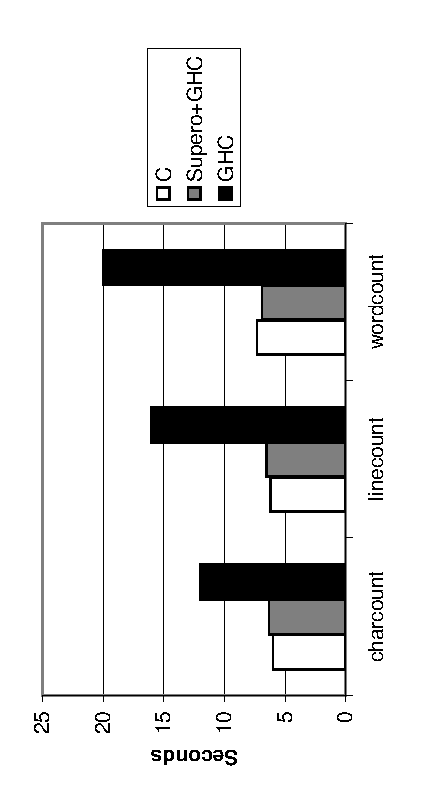
\includegraphics[scale=0.75,angle=270]{wc.eps}
\end{center}
\vspace{1mm}
\figend
\caption{Benchmarks with C, Supero+GHC and GHC alone.}
\label{fig:c_results}
\end{fig}

The results are given in Figure \ref{fig:c_results}. In all the benchmarks C and Supero are within 10\% of each other, while GHC trails further behind.

\subsection{Identified Haskell Speedups}

During initial trials using these benchmarks, we identified two unnecessary bottlenecks in the Haskell version of word counting. Both were remedied before the presented results were obtained.

\paragraph{Slow \textsf{isSpace} function}

The first issue is that |isSpace| in Haskell is much more expensive than |isspace| in C. The simplest solution is to use a FFI (Foreign Function Interface) \cite{spj:awkward_squad} call to the C |isspace| function in all cases, removing this factor from the benchmark. A GHC bug (number 1473) has been filed about the slow performance of |isSpace|.

\begin{fig}
\begin{code}
words :: String -> [String]
words s = case  dropWhile isSpace s of
                []  ->  []
                x   ->  w : words y
                        where (w, y) = break isSpace x

words' s = case  dropWhile isSpace s of
                 []    ->  []
                 x:xs  ->  (x:w) : words' (drop1 z)
                           where (w, z) = break isSpace xs

drop1 []      = []
drop1 (x:xs)  = xs
\end{code}
\figend
\caption{The |words| function from the Haskell standard libraries, and an improved |words'|.}
\label{fig:words}
\end{fig}

\paragraph{Inefficient \textsf{words} function}

The second issue is that the standard definition of the |words| function (given in Figure \ref{fig:words}) performs two additional |isSpace| tests per word. By appealing to the definitions of |dropWhile| and |break| it is possible to show that in |words| the first character of |x| is not a space, and that if |y| is non-empty then the first character is a space. The revised |words'| function uses these facts to avoid the redundant |isSpace| tests.

\subsection{Potential GHC Speedups}

% NOTE: Shorten this section if space needed

We have identified three factors limiting the performance of residual programs when compiled by GHC. These problems cannot be solved at the level of Core transformations. We suspect that by fixing these problems, the Supero execution time would improve by between 5\% and 15\%.

\paragraph{Strictness inference}

The GHC compiler is overly conservative when determining strictness for functions which use the FFI (GHC bug 1592). The |getchar| function is treated as though it may raise an exception, and terminate the program, so strict arguments are not determined to be strict. If GHC provided some way to mark an FFI function as not generating exceptions, this problem could be solved. The lack of strictness information means that in the line and word counting programs, every time the accumulator is incremented, the number is first unboxed and then reboxed \cite{spj:unboxing}.

\paragraph{Heap checks}

The GHC compiler follows the standard STG machine \cite{spj:implementation} design, and inserts heap checks before allocating memory. The purpose of a heap check is to ensure that there is sufficient memory on the heap, so that allocation of memory is a cheap operation guaranteed to succeed. GHC also attempts to lift heap checks: if two branches of a case expression both have heap checks, they are replaced with one shared heap check before the case expression. Unfortunately, with lifted heap checks, a tail-recursive function that allocates memory only upon exit can have the heap test executed on every iteration (GHC bug 1498). This problem affects the character counting example, but if the strictness problems were solved, it would apply equally to all the benchmarks.

\paragraph{Stack checks}

The final source of extra computation relative to the C version are stack checks. Before using the stack to store arguments to a function call, a test is performed to check that there is sufficient space on the stack. Unlike the heap checks, it is necessary to analyse a large part of the flow of control to determine when these checks are unnecessary. It is not clear how to reduce stack checks in GHC.

\begin{comment}
\subsection{Why Supero Outperforms C for the Wordcount Benchmark}

The most curious result is that Supero outperforms C on wordcounting, by about 6\% -- even with the problems discussed! The C program presented in Figure \ref{fig:c_words} is not optimal. The variable \verb"last_space" is a boolean, indicating whether the previous character was a space, or not. Each time round the loop a test is performed on \verb"last_space", even though its value was determined and tested on the previous iteration. The way to optimise this code is to have two specialised variants of the loop, one for when \verb"last_space" is true, and one for when it is false. When the value of \verb"last_space" changes, the program would transition to the other loop. This pattern effectively encodes the boolean variable in the program counter, and is what the Haskell program has managed to generate from the high-level code.

However, in C it is quite challenging to capture the required control flow. The program needs two loops, where both loops can transition to the other. Using \texttt{goto} turns off many critical optimisations in the C compiler. Tail recursion is neither required by the C standard, nor supported by most compilers. The only way to express the necessary pattern is using nested while loops, but unlike newer imperative languages such as Java, C does not have named loops -- so the inner loop cannot break from the outer loop if it reaches the end of the file. The only solution is to place the nested while loops in a function, and use \texttt{return} to break from the inner loop. This solution would not scale to a three-valued control structure, and substantially increases the complexity of the code.
\end{comment}

\section{Performance Compared With GHC Alone}
\label{sec:haskell_results}

The standard set of Haskell benchmarks is the nofib suite \cite{nofib}. It is divided into three categories of increasing size: imaginary, spectral and real. Even small Haskell programs increase in size substantially once libraries are included, so we have limited our attention to the benchmarks in the imaginary section. All benchmarks were run with parameters that require runtimes of between 3 and 5 seconds for GHC.

We exclude two benchmarks, paraffins and gen\_regexps. The paraffins benchmark makes substantial use of arrays, and we have not yet mapped the array primitives of Yhc onto those of GHC, which is necessary to run the transformed result. The gen\_regexps benchmark tests character processing: for some reason (as yet unknown) the supercompiled executable fails.

\begin{fig}
\vspace{4mm}
\begin{center}
% http://csdl.ics.hawaii.edu/FAQ/chart-ps.html
\includegraphics[scale=0.75,angle=270]{nofib.eps}
\end{center}
\vspace{3mm}
\figend
\caption{Runtime, relative to GHC being 1.}
\label{fig:haskell_results}
\end{fig}

\begin{table}[tb]
\hrule
\vspace{3mm}

\begin{tabular}{lrrrrrr}
\textbf{Program} & \hspace{5mm}\textbf{Supero} & \hspace{5mm}\textbf{msg} & \hspace{5mm}\textbf{spine} & \hspace{5mm}\textbf{none} & \hspace{5mm}\textbf{Size} & \hspace{5mm}\textbf{Memory} \\
bernouilli 		& 1.41 & 1.53 & 1.58 & 1.18 & 1.10 & 0.97 \\
digits-of-e1	& 1.03 & 1.16 & 1.03 & 1.06 & 1.01 & 1.11 \\
digits-of-e2	& 0.72 & 0.72 & 0.72 & 1.86 & 1.00 & 0.84 \\
exp3\_8			& 1.00 & 1.00 & 1.00 & 1.01 & 0.99 & 1.00 \\
integrate 		& 0.46 & 0.47 & 0.46 & 4.01 & 1.02 & 0.08 \\
primes 			& 0.57 & 0.57 & 0.88 & 0.96 & 1.00 & 0.98 \\
queens 			& 0.79 & 0.96 & 0.83 & 1.21 & 1.01 & 0.85 \\
rfib 			& 0.97 & 0.97 & 0.97 & 1.00 & 1.00 & 1.08 \\
tak 			& 0.72 & 1.39 & 1.39 & 1.39 & 1.00 & 1.00 \\
wheel-sieve1 	& 0.98 & 1.11 & 1.42 & 5.23 & 1.19 & 2.79 \\
wheel-sieve2 	& 0.87 & 0.63 & 0.89 & 0.63 & 1.49 & 2.30 \\
x2n1 			& 0.58 & 0.64 & 1.61 & 3.04 & 1.09 & 0.33 \\
\end{tabular}
\vspace{2mm}

\textbf{Program} is the name of the program; \textbf{Supero} uses the $\bowtie$ generalisation method; \textbf{msg} uses the msg function for generalisation; \textbf{spine} applies no generalisation operation; \textbf{none} never performs any inlining; \textbf{Size} is the size of the Supero generated executable; \textbf{Memory} is the amount of memory allocated on the heap by the Supero executable.

\vspace{4mm}
\hrule
\vspace{2mm}
\caption{Runtime, relative to GHC being 1.}
\label{tab:haskell_results}
\end{table}

The results of these benchmarks are given in Figure \ref{fig:haskell_results}, along with detailed breakdowns in Table \ref{tab:haskell_results}. All results are relative to the runtime of a program compiled with GHC -O2, lower numbers being better. The first three variants (Supero, msg, spine) all use homeomorphic embedding as the termination criterion, and $\bowtie$, msg or nothing respectively as the generalisation function. The final variant, none, uses a termination test that always causes a residuation. The `none' variant is useful as a control to determine which improvements are due to bringing all definitions into one module scope, and which are a result of supercompilation. Compilation times ranged from a few seconds to five minutes.

The Bernouilli benchmark is the only one where Supero is slower than GHC by more than 3\%. The reason for this anomaly is that a dictionary is referred to in an inner loop which is specialised away by GHC, but not by Supero.

With the exception of the wheel-sieve2 benchmark, our $\bowtie$ generalisation strategy performs as well as, or better than, the alternatives. While the msg generalisation performs better than the empty generalisation on average, the difference is not as dramatic.

\subsection{GHC's optimisations}

For these benchmarks it is important to clarify which optimisations are performed by GHC, and which are performed by Supero. The `none' results show that, on average, taking the Core output from Yhc and compiling with GHC does \textit{not} perform as well as the original program compiled using GHC. GHC has two special optimisations that work in a restricted number of cases, but which Supero produced Core is unable to take advantage of.

\paragraph{Dictionary Removal} Functions which make use of type classes are given an additional dictionary argument. In practice, GHC specialises many such functions by creating code with a particular dictionary frozen in. This optimisation is specific to type classes -- a tuple of higher order functions is not similarly specialised. After compilation with Yhc, the type classes have already been converted to tuples, so Supero must be able to remove the dictionaries itself. One benchmark where dictionary removal is critical is digits-of-e2.

\paragraph{List Fusion} GHC relies on names of functions, particularly |foldr|/|build| \cite{spj:rules}, to apply special optimisation rules such as list fusion. Many of GHC's library functions, for example |iterate|, are defined in terms of |foldr| to take advantage of these special properties. After transformation with Yhc, these names are destroyed, so no rule based optimisation can be performed. One example where list fusion is critical is primes, although it occurs in most of the benchmarks to some extent.

\begin{comment}
\subsection{Termination Bound}
\label{sec:results_bound}

Table \ref{tab:haskell_results} includes a column indicating the size bound that was applied to expressions. Out of the five benchmarks, both primes and queens could be run at any greater bound and would still produce the same program -- the direct repetition criteria (see \S\ref{sec:direct}) bounds the expressions on its own. For the remaining programs, a bound was chosen to ensure that the compilation process was quick (under two seconds). By increasing the termination bound the size of the residual program would increase, but the generated program may execute faster.

The existence of a termination bound requiring different values for different programs is a cause for concern. In a large program it is likely that different parts of the program would require different bounds on the size of the generated expression -- something not currently possible. We suspect that the most promising direction is to augment the direct repetition criterion to obtain termination in all practical cases without resorting to a depth bound.
\end{comment}

\section{Related Work}
\label{sec:related}

Supercompilation \cite{supercompilation,turchin:experiments} was introduced by Turchin for the Refal language \cite{refal}. Since this original work, there have been various suggestions of both termination strategies and generalisation strategies \cite{turchin:generalisation,sorensen:supercompilation,leuschel:homeomorphic}. The original supercompiler maintained both positive and negative knowledge, but our implementation is a simplified version maintaining only positive information \cite{secher:perfect_supercompilation}.

The issue of let expressions in supercompilation has not previously been a primary focus. If lets are mentioned, the usual strategy is to substitute all linear lets and residuate all others. Lets have been considered in a strict setting \cite{jonsson:supercompilation}, where they are used to preserve termination semantics, but in this work all strict lets are inlined without regard to loss of sharing. Movement of lets can have a dramatic impact on performance: carefully designed let-shifting transformations give an average speedup of 15\% in GHC \cite{spj:letfloating}, suggesting let expressions are critical to the performance of real programs.

\paragraph{Partial evaluation} There has been a lot of work on partial evaluation \cite{jones:partial_evaluation}, where a program is specialised with respect to some static data. The emphasis is on determining which variables can be entirely computed at compile time, and which must remain in the residual program. Partial evaluation is particularly appropriate for specialising an interpreter with an expression tree to generate a compiler automatically, often with an order of magnitude speedup, known as the First Futamura Projection \cite{futanama:projections}. Partial evaluation is not usually able to remove intermediate data structures. Our method is certainly less appropriate for specialising an interpreter, but in the absence of static data, is still able to show improvements.

% Partial evaluation has been applied to full-scale functional languages, such as Curry
% \cite{albert:partial_evaluation_curry}.

\paragraph{Deforestation} The deforestation technique \cite{wadler:deforestation} removes intermediate lists in computations. This technique has been extended in many ways to encompass higher order deforestation \cite{marlow:higher_order_deforestation} and work on other data types \cite{coutts:string_fusion}. Probably the most practically motivated work has come from those attempting to restrict deforestation, in particular shortcut deforestation \cite{gill:shortcut_deforestation}, and newer approaches such as stream fusion \cite{coutts:stream_fusion}. In this work certain named functions are automatically fused together. By rewriting library functions in terms of these special functions, fusion occurs.

\paragraph{Whole Program Compilation} The GRIN approach \cite{grin} uses whole program compilation for Haskell. It is currently being implemented in the jhc compiler \cite{jhc}, with promising initial results. GRIN works by first translating Haskell into a monadic intermediate language, then repeatedly performing a series of optimisations, upon the whole program at once. The intermediate language is at a much lower level than our Core language, so jhc is able to perform detailed optimisations that we are unable to express.

\paragraph{Lower Level Optimisations} Our optimisation works at the Core level, but even once efficient Core has been generated there is still some work before efficient machine code can be produced. Key optimisations include strictness analysis and unboxing \cite{spj:unboxing}. In GHC both of these optimisations are done at the Core level, using a Core language extended with unboxed types. After this lower level Core has been generated, it is then compiled to STG machine instructions \cite{spj:stg}, from which assembly code is generated. There is still work being done to modify the lowest levels to take advantage of the current generation of microprocessors \cite{marlow:pointer_tagging}. We rely on GHC to perform all these optimisations after Supero generates a residual program.

\begin{comment}
\paragraph{Other Transformations} One of the central operations within our optimisation in inlining, a technique that has been used extensively within GHC \cite{spj:inlining}. We generalise the constructor specialisation technique \cite{spj:specconstr}, by allowing specialisation on any arbitrary expression, including constructors.

One optimisation we do not currently support is the use of user provided transformation rules \cite{spj:rules}, which can be used to automatically replace certain expressions with others -- for example |sort . nub| removes duplicates then sorts a list, but can be done asymptotically faster in a single operation.
\end{comment}

\section{Conclusions and Future Work}
\label{sec:conclusion}

Our supercompiler is simple -- the Core transformation is expressed in just 300 lines of Haskell. Yet it replicates many of the performance enhancements of GHC in a more general way. We have modified some of the techniques from supercompilation, particularly with respect to let bindings and generalisation. Our initial results are promising, but incomplete. Using our supercompiler in conjunction with GHC we obtain an average runtime improvement of 16\% for the imaginary section of the nofib suite. To quote Simon Peyton Jones, ``an average runtime improvement of 10\%, against the baseline of an already well-optimised compiler, is an excellent result'' \cite{spj:specconstr}.

There are three main areas for future work:

\begin{description}
\item[More Benchmarks] The fifteen benchmarks presented in this paper are not enough. We would like to obtain results for larger programs, including all the remaining benchmarks in the nofib suite.
\item[Runtime Performance] Earlier versions of Supero \cite{me:supero_ifl} managed to obtain substantial speed ups on benchmarks such as exp3\_8. The Bernouilli benchmark is currently problematic. There is still scope for improvement.
\item[Compilation Speed] The compilation times are tolerable for benchmarking and a final optimised release, but not for general use. Basic profiling shows that over 90\% of supercompilation time is spent testing for a homeomorphic embedding, which is currently done in a na\"{i}ve manner -- dramatic speedups should be possible.
\end{description}

The Programming Language Shootout\footnote{\url{http://shootout.alioth.debian.org/}} has shown that low-level Haskell can compete with low-level imperative languages such as C. Our goal is that Haskell programs can be written in a high-level declarative style, yet still perform competitively.

\paragraph{Acknowledgements} We would like to thank Simon Peyton Jones, Simon Marlow and Tim Chevalier for help understanding the low-level details of GHC, and Peter Jonsson for helpful discussions and presentation suggestions.

\bibliographystyle{plain}

\bibliography{supero}

\end{document}
